\section{Detailed Design}
\label{Section: design}

\begin{figure*}[!t]
	%\begin{tabular}{cc}
	\begin{minipage}{\linewidth}
		\centerline{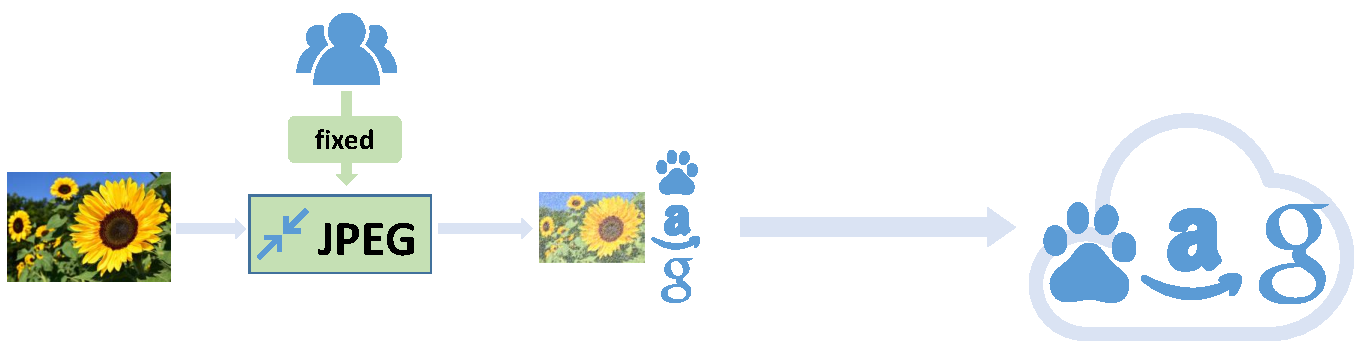
\includegraphics[width=0.8\linewidth]{figures/conventional-framework.pdf}}
		\begin{center}
			{(a) Conventional solution: fixed user-defined compression quality level}
		\end{center}
		%        \vspace{0.3cm}
	\end{minipage}
	\vfill
	\vspace{0.4cm}
	\begin{minipage}{\linewidth}
		\centerline{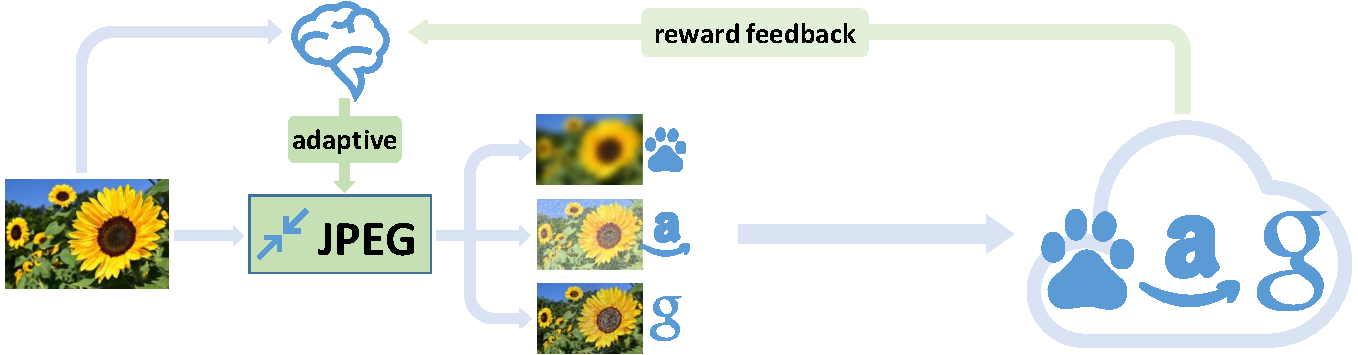
\includegraphics[width=0.8\linewidth]{figures/adaptive-framework.pdf}}
		\vspace{0.2cm}
		\begin{center}
			{(b) AdaCompress solution: input image and model aware compression}
		\end{center}
	\end{minipage}
	%\end{tabular}
	%\vspace{0.1cm}
	\caption{Comparing to the conventional solution, our solution can update the compression strategy based on the backend model feedback}
	\label{fig: framework}
\end{figure*}

A brief framework of AdaCompress is shown in Figure~\ref{fig: framework}. Briefly, it is a reinforcement learning-based system to train an agent to choose a proper compression quality level $ c $ for one image to be compressed by JPEG. We discuss the formulation, agent design, reinforcement learning-based framework, reward feedback, \emph{inference-estimation-querying-retraining} mechanism, and insight of RL agent's behaviors separately in the following subsections. We provide experimental details of all the hyperparameters in Section.~\ref{Section: evaluation}. %% \\

\subsection{Problem Formulation}
\label{subsec: formulation}

% \colorbox{red}{notation table}
Without loss of generality, we denote the cloud-based deep learning service as $ \vec{y}_i = M(x_i) $ that provides a predicted result list $ \vec{y}_i $ for each input image $ x_i $. It has a baseline output $ \vec{y}_{\rm ref} = M(x_{\rm ref}) $ for each reference input image $ x \in X_{\rm ref} $. We use this $ \vec{y}_{\rm ref} $ as the ground truth label. For each image $ x_c $ compressed at compression quality level $ c $, the output $ \vec{y}_c = M(x_c) $. Therefore, we have an accuracy metric $ \mathcal{A}_c $ by comparing $ \vec{y}_{\rm ref} $ and $ \vec{y}_c $. In general, we use the top-5 accuracy as the following $ \mathcal{A} $, the same as the classification metric of ILSVRC2012~\cite{ILSVRC12}.

\begin{align}
\mathcal{A} =& \frac{1}{k} \sum_{k}\max_jd(l_j, g_k) \\
& l_j \in \vec{y}_c, \quad j=1,...,5 \\
& g_k \in \vec{y}_{\rm ref}, \quad k=1, ..., {\rm length}(\vec{y}_{\rm ref}) \\
& d(x, y) = 1 \ \text{if} \ x=y  \ \text{else} \ 0 
\end{align}

Where $ j = 1,...,5 $ indicates the prediction labels at the top-5 score, meaning that if any one of the top-5 predicted labels matches the ground truth label $ \vec{y}_{\rm ref} $, it would be regarded as a correct prediction. In general, we cannot get the cloud-based deep learning model's in-layer details (e.g., softmax probabilities) for a cloud-based deep learning service. Therefore we use a binary hard label $ d(x, y) \in \{0, 1\} $ to evaluate the accuracy. %% $ d(x, y) \in \{0, 1\} $

We also denote JPEG input images as $ f_{ic} = J(x_i, c) $ that for an input image $ x_i $ and a given compression quality level $ c $, and it outputs a compressed file $ f_{ic} $ at the size of $ s_{ic} $. For a reference compression quality level $ c_{\rm ref} $, the compressed file size is $ s_{\rm ref} $. Besides, the input image from a specific scenery usually belongs to a particular contextual group~\cite{mcdnn}. For example, in the daytime, the input images are expected to have a bright background, while nighttime images are usually gray-scaled thermal images. Therefore, the agent in one scenery does not need to know all the contextual features in all ``sceneries''. We formulate this as contextual group $ \mathcal{X} $.
%This contextual grouping concept is also discussed in~\cite{mcdnn}.

Initially, the agent tries different compression quality levels $ c_{\min} < c < c_{\max}, c \in \mathbb{N} $ to obtain compressed image $ x_c $ from input image $ x $. To obtain cloud-end recognition results $ \{\vec{y}_{\rm ref}, \vec{y}_c\} $, the agent uploads the compressed image $ x_c $ and the reference image $ x_{\rm ref} $ to the cloud-end. Comparing the two uploaded instances $ \{x_{\rm ref}, x_c\} $ and cloud-end recognition results $ \{\vec{y}_{\rm ref}, \vec{y}_c\} $, the agent obtains the reference file size $ s_{\rm ref} $ and compressed file size $ s_c $, and computes the file compression ratio $ \Delta s = \frac{s_c}{s_{\rm ref}} $ and accuracy metric $ \mathcal{A}_c $.

\subsection{RL Agent Design}

The RL agent is expected to give a proper compression quality level $ c $ for minimizing the file size $ s_c $ while keeping the accuracy $ \mathcal{A} $. For the RL agent, the input features are continuous numerical vectors, and the expected output is discrete compression quality level $ c $. Therefore we can use the Deep Q-learning Network as the RL agent. But the naive Deep Q-learning Network can not work well in this task because of the following challenges: %% \\

\begin{itemize}
	\item The state space of reinforcement learning is too large. To preserve enough details, we have to add many layers and nodes to the neural network, making the RL agent extremely difficult to converge. 
	\item It takes a long time to train one step in a large inference neural network, making the training process too time-consuming.
	\item The RL agent starts training from random trials and learns afterward from the reward feedback. When training from a randomly initialized neural network, the reward feedback is very sparse, making it difficult for the agent to learn.
\end{itemize}

To address these challenges, we use the early layers of a pre-trained neural network to extract the structural information of an input image. This is a commonly used strategy in training a deep neural network~\cite{finetunning,finetunning2}. Therefore instead of training a RL agent directly from the input image, we use a pre-trained small neural network to extract the features from the input image to reduce the input dimension and accelerate the training procedure. In this work, we use the early convolution layers of MobileNetV2~\cite{MobileNetV2} as the image feature extractor $ \mathcal{E}(\cdot) $ for its efficiency in image classification. The Deep Q-learning Network $ \phi $ is connected to the feature extractor's last convolution layer. We update the RL agent's policy by changing the parameters of the Deep Q-learning Network $ \phi $ while fixing the feature extractor $ \mathcal{E} $. %% \\

\subsection{Reinforcement Learning-based Framework}

In a specific scenery where the user input image $ x $ belongs to the contextual group $ \mathcal{X} $, we define the contextual group $ \mathcal{X} $, along with the backend cloud model $ M $, as the \emph{emulator environment} $ \{\mathcal{X}, M\} $ of the reinforcement learning problem. 

We formulate the feature extractor's output $ \mathcal{E}(J(\mathcal{X}, c)) $ as \emph{states} and the compression quality level $ c $ as discrete \emph{actions}. In our system, to accelerate training, we define 10 discrete actions to indicate 10 compression quality levels of JPEG ranging from $ 5, 15, ...,95 $. We denote the \emph{action-value function} as $ Q(\phi(\mathcal{E}(f_t)), c; \theta) $ and the optimal compression quality level at time $ t $ as $ c_t = {\rm argmax}_cQ(\phi(\mathcal{E}(f_t)), c; \theta) $ where $ \theta $ indicates the parameters of the Deep Q-learning Network $ \phi $. In such reinforcement learning formulation, the training phase is to minimize the loss function $ L_i(\theta_i) = \mathbb{E}_{s, c \sim \rho (\cdot)}\Big[\big(y_i - Q(s, c; \theta_i)\big)^2 \Big] $ that changes at each iteration $ i $ where $ s = \mathcal{E}(f_t) $ and target $ y_i = \mathbb{E}_{s' \sim \{\mathcal{X}, M\}} \big[ r + \gamma \max_{c'} Q(s', c'; \theta_{i-1}) \mid s, c \big] $. Especially, $ r $ is the reward feedback, and $ \rho(s, c) $ is a probability distribution over sequences $ s $ and the compression quality level $ c $~\cite{DQN}. When minimizing the distance of \emph{action-value function}'s output $ Q(\cdot) $ and target $ y_i $, the \emph{action-value function} $ Q(\cdot) $ outputs a more accurate estimation of an action. 

Different from conventional reinforcement learning, the interactions between the agent and environment are infinite, i.e., there is no signal from the environment telling that an episode has finished. Therefore, we train the RL agent intermittently at a manual interval of $ T $ after the condition $ t \geq T_{\rm start} $ guaranteeing that there are enough transitions in the memory buffer $ \mathcal{D} $. In the training phase, the RL agent firstly takes some random trials to observe the environment's reaction and decreases the randomness when training afterward. All transitions are saved into a memory buffer $ \mathcal{D} $, and the agent learns to optimize its \emph{action} by minimizing the loss function $ L $ on a mini-batch from $ \mathcal{D} $. The training procedure would converge when the agent's randomness keeps decaying. Finally, the agent's action is based on its historical ``optimal'' experiences. The training procedure is presented in Algorithm~\ref{alg: rl-train}.
% and we list the parameters in Section.~\ref{Section: evaluation}.

\begin{algorithm}[!t]
	\caption{Training RL agent $ \phi $ in environment $ \{\mathcal{X}, M\} $}
	\label{alg: rl-train}
	\begin{algorithmic}[1]
		\STATE Initialize replay memory buffer $ \mathcal{D} $ to capacity $ N $
		\STATE Initialize \emph{action-value function} $ Q $ with random weights $ \theta $
		\STATE Initialize sequence $ s_1 = \mathcal{E}\big(J(x_1, c_1)\big), x_1 \in \mathcal{X} $ and $ \phi_1 = \phi(f_1) $
		\FOR {$t \in 1,2,\cdots, K$}
%		\STATE \textbf{1) Exploration.} %With probability $\epsilon$:
		{\color{revise}\STATE \textbf{1) Exploration}}
		{\color{revise}\STATE With probability $\epsilon$:}
		\STATE \hspace{1em} $c_t \leftarrow$ a random valid value 
		\STATE Otherwise:
		\STATE \hspace{1em} $ c_t \leftarrow {\rm argmax}_cQ\Big(\phi\big(\mathcal{E}(f_t)\big), c; \theta\Big) $

		\STATE
		
%		\STATE \textbf{2) Reward calcuation.} 
		{\color{revise}\STATE \textbf{2) Reward calcuation}} 
		\STATE Compress image $ x_t $ at quality $ c_t $ to upload
		\STATE Receive $ (\vec{y}_{\rm ref}, \vec{y}_c) $ from the cloud service
		\STATE $ r \leftarrow R(\Delta s, \mathcal{A}_c) $
		
		\STATE 
%		\STATE \textbf{3) Gradient decent.} %Generate $ c_t, x_{t+1} $
		{\color{revise}\STATE \textbf{3) Gradient decent}}
		{\color{revise}\STATE Generate $ c_t, x_{t+1} $}
		\STATE $ s_{t+1} \leftarrow s_t $, $ \phi_{t+1} \leftarrow \phi \big(\mathcal{E}(f_{t+1})\big) $
		\STATE $ \mathcal{D} \leftarrow \mathcal{D} \bigcup \{(\phi_t, c_t, r_t, \phi_{t+1}) \} $
		\IF {$ t \mod T = 0 $ and $ t \geq T_{\rm start} $}
%		\STATE Sample a randomly mini-batch of transitions \\ $ (\phi_j, c_j, r_j, \phi_{j+1}) $ from memory buffer $ \mathcal{D} $
		{\color{revise}
		\STATE Sample a randomly mini-batch of transitions $ (\phi_j, c_j, r_j, \phi_{j+1}) $ from memory buffer $ \mathcal{D} $
		\STATE $ y_i \leftarrow r_j + \gamma \max_{c'}Q(\phi_{j+1}, c'; \theta) $
		\STATE Compute decay exploration rate 
		$ \epsilon \leftarrow 
		\begin{cases}
		\mu_{\rm dec}\cdot \epsilon & \text{ if } \ \mu_{\rm dec}\cdot \epsilon > \epsilon_{\min} \\ 
		\epsilon_{\min}             & \text{ if } \ \mu_{\rm dec}\cdot \epsilon \leq \epsilon_{\min}
		\end{cases} $
		\STATE Perform a gradient descent step on $ \big(y_j - Q(\phi_j, c_j; \theta)\big)^2 $ according to~\cite{DQN}
		}
%		\STATE Perform a gradient descent step on \\ $ \big(y_j - Q(\phi_j, c_j; \theta)\big)^2 $ according to~\cite{DQN}
		\ENDIF
		\ENDFOR
	\end{algorithmic}
\end{algorithm}

\subsection{Reward Feedback Design}

In our solution, the agent is trained by the reward feedback from the environment $ \{\mathcal{X}, M\} $. In the above formulation, we define compression rate $ \Delta s = \frac{s_c}{s_{\rm ref}} $ and accuracy metric $ \mathcal{A}_c $ at compression quality level $ c $. Basically, we want the agent to choose a proper compression quality level for minimizing the upload image size while remaining acceptable accuracy. \textcolor{revise}{Therefore the overall reward $ r $ should be positively correlated with the accuracy $ \mathcal{A} $ while negatively with the compression ratio $ \Delta s $.} We introduce two linear factors $ \alpha $ and $ \beta $ to form a linear combination $ r = \alpha \mathcal{A} - \Delta s + \beta $ as the \emph{reward function} $ R(\Delta s, \mathcal{A}) $. %% \\

% Therefore the overall reward $ r $ should be in proportion to the accuracy $ \mathcal{A} $ while in inverse proportion to the compression ratio $ \Delta s $.
\subsection{Inference-Estimation-Querying-Retraining Mechanism}

As a running system, we introduce an \emph{inference-estimation-querying-retraining} mechanism to cope with the scenery change in the inference phase, building a system with different components to inferring, capturing the scenery change, then either re-loading or re-training the RL agent based on the performance of the cached model. The overall system diagram is illustrated in Figure~\ref{fig: diagram}.

%\begin{figure}[H]
%    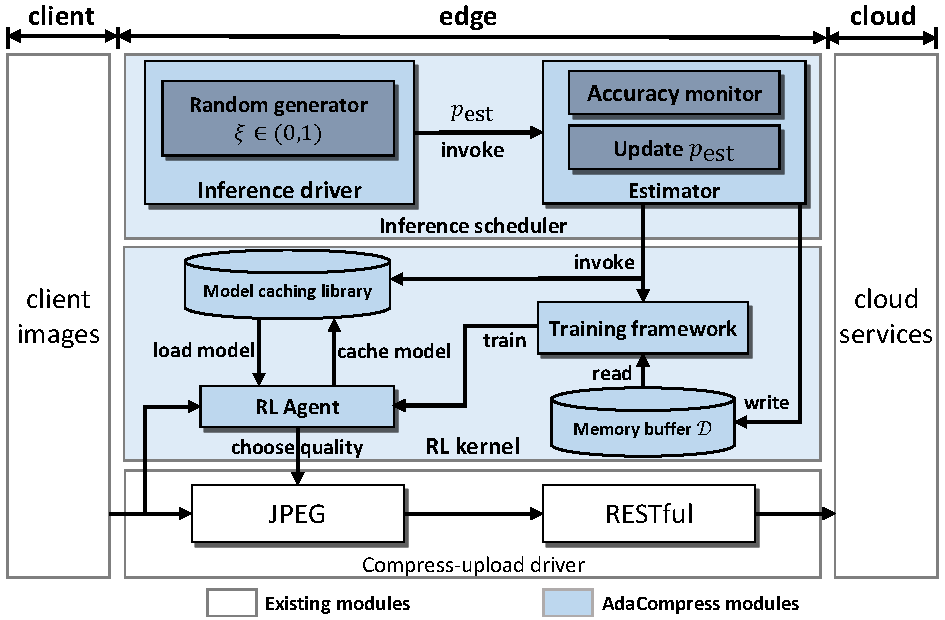
\includegraphics[width=\linewidth]{figures/overall-diagram.pdf}
%    \caption{Diagram of AdaCompress architecture}
%    \label{fig: diagram}
%\end{figure}

\begin{figure}[!t]
	\centerline{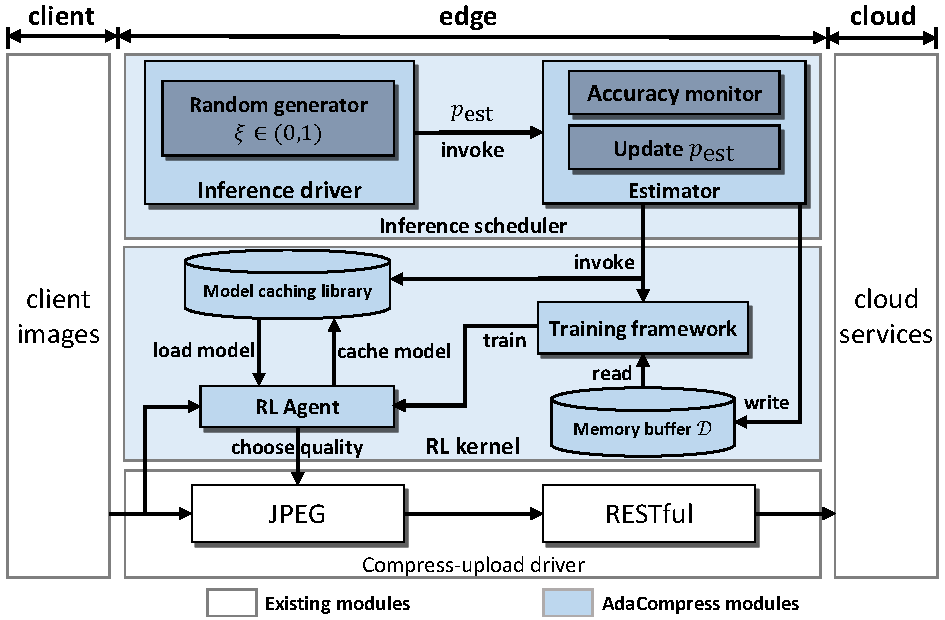
\includegraphics[width=0.8\linewidth]{figures/overall-diagram.pdf}}
%	\vspace{0.2cm}
	\caption{Diagram of AdaCompress architecture}
	\label{fig: diagram}
\end{figure}

%\begin{figure}[H]
%	\centerline{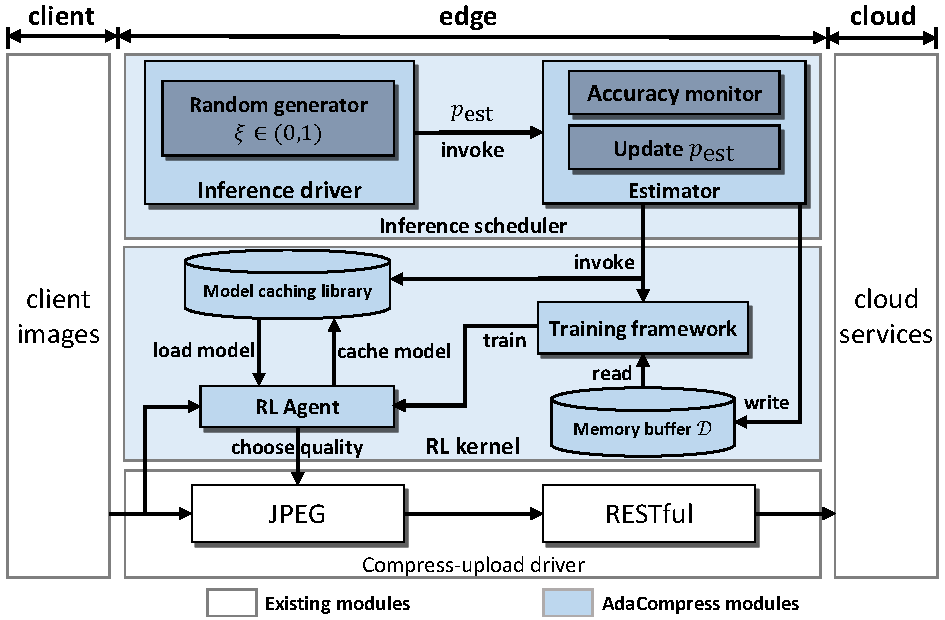
\includegraphics[width=0.8\linewidth]{figures/overall-diagram.pdf}}
%	\vspace{0.2cm}
%	\caption{Diagram of AdaCompress architecture}
%	\label{fig: diagram}
%\end{figure}

%% The system diagram is shown in Figure~\ref{fig: diagram}.
We build up the memory buffer $ \mathcal{D} $ and reinforcement learning training kernel based on the compression and upload driver. When the RL training kernel is called, it would load transitions from the memory buffer $ \mathcal{D} $ to train the compression quality level predictor $ \phi $. When the system is deployed, the pre-trained RL agent $ \phi $ guides the compression driver to compress the input image at an adaptive compression quality level $ c $, then uploads the compressed image to cloud-end. %% \\

After the AdaCompress is deployed, the input image scenery context $ \mathcal{X} $ may change (e.g., day to night, sunny to rainy). When the scenery changes, the older RL agent's compression selection strategy may not be suitable anymore, causing the overall accuracy to decrease. To cope with the scenery change, AdaCompress invokes an estimator with a probability $ p_{\rm est} $. AdaCompress does this by generating a random value $ \xi \in (0,1) $ and comparing it to $ p_{\rm est} $. If $ \xi \leq p_{\rm est} $, the estimator would be invoked. AdaCompress would upload the reference image $ x_{\rm ref} $ along with the compressed image $ x_i $ to obtain $ \vec{y}_{\rm ref} $ and $ \vec{y}_i $, calculate $ \mathcal{A}_i $ and save the transition $ (\phi_i, c_i, r_i, \mathcal{A}_i) $ to the memory buffer $ \mathcal{D} $. The estimator also compares the recent $ n $ steps' average accuracy $ \bar{\mathcal{A}}_n $ and the initial accuracy threshold $ \mathcal{A}_0 $. Once the recent average accuracy is lower than the initial accuracy threshold, the estimator would query a RL agent model to replace the current agent model and test the performance of the loaded model. To test the loaded model's performance, the estimator computes the average accuracy $ \bar{\mathcal{A}}^*_n $. If $ \bar{\mathcal{A}}^*_n $ is still lower than the accuracy threshold, the estimator would invoke the RL training kernel to re-train the agent. Once the estimator discovers that the trained reward is higher than the reward threshold, it would stop the training kernel, cache the trained RL agent, and switch to the normal inference state. 

Since the reference image $ x_{\rm ref} $ and the compressed image $ x_i $ are both needed in the re-training phase, causing a large upload image size overhead, especially when the scenery changes frequently (e.g., day to night, then night to day). To avoid unnecessary upload traffic load in the re-training phase, we build up the model caching library to cache the trained RL agent models. When capturing the scenery change, we firstly query a pre-trained model from the model caching library rather than re-training from scratch. %% \\

The \emph{inference-estimation-querying-retraining} mechanism has four states, including inference, estimation, model querying and re-training. AdaCompress switches to these states adaptively. The state switching policy is shown as Figure~\ref{fig: state-switching}.
%\begin{figure}[H]
%    \begin{tikzpicture}[->,>=stealth',shorten >=1pt,auto,node distance=1.8cm, semithick]
%    \tikzstyle{every state}=[ellipse, align=center, draw=blue, text=black]
%    
%    \node[initial, state] (B)                    {inference};
%    \node[state]         (C) [below right of=B] {re-train};
%    \node[state]         (D) [above right of=C] {estimate};
%    
%    \path   (B) edge [loop above] node {$ \xi > p_{\rm est} $} (B)
%    (B.10)    edge                node {$ \xi \leq p_{\rm est} $} (D.170)
%    (C) edge [below left]      node {$ \bar{r}_n > r_{\rm th} $} (B)
%    edge [loop below] node {$ \bar{r}_n \leq r_{\rm th} $}     (C)
%    (D) edge [loop right] node {$ \xi \leq p_{\rm est} $} (D)
%    (D.190)    edge              node {$ \xi > p_{\rm est} $} (B.-10)
%    (D.225)    edge [below right]      node {$ \bar{\mathcal{A}_n} < \mathcal{A}_0 $} (C);
%    \end{tikzpicture}
%    % \vspace{-0.3cm}
%    \caption{State switching policy}
%    \label{fig: state-switching}
%    %\vspace{-0.8cm}
%\end{figure}
\begin{figure}[!t]
	\begin{tikzpicture}[->,>=stealth',shorten >=1pt,auto,node distance=2.1cm, semithick]
	\tikzstyle{every state}=[ellipse, align=center, draw=blue, text=black]
	
	\node[initial, state] (B)                    {inference};
	\node[state]         (C) [below of=B] {re-training};
	\node[state]         (D) [right of=B, node distance=4cm] {estimation};
	\node[state]         (E) [right of=C, node distance=4cm] {model querying};
	%    \node[state][rectangle]   (F) [below right of=C, node distance=2.5cm] {Model Library};
	
	\path   (B) edge [loop above] node {$ \xi > p_{\rm est} $} (B)
	(B.10)    edge                node {$ \xi \leq p_{\rm est} $} (D.170)
	(C) edge [below left]      node {$ \bar{r}_n > r_{\rm th} $} (B)
	edge [loop below] node {$ \bar{r}_n \leq r_{\rm th} $}     (C)
	(D) edge [loop above] node {$ \xi \leq p_{\rm est} $} (D)
	(D.190)    edge              node {$ \xi > p_{\rm est} $} (B.-10)
	(D)    edge [below right]      node {$ \bar{\mathcal{A}_n} < \mathcal{A}_0 $} (E)
	(E) edge [below left] node [left] {$ \bar{\mathcal{A}^*_n} \geq \mathcal{A}_0 $} (B)
	(E) edge [below left] node [below] {$ \bar{\mathcal{A}^*_n} < \mathcal{A}_0 $} (C);
	%    (C) edge [below right] node [left] {cache model} (F)
	%    (F) edge [below right] node [right] {load model} (E);
	\end{tikzpicture}
	% \vspace{-0.3cm}
	\caption{State switching policy}
	\label{fig: state-switching}
	%\vspace{-0.8cm}
\end{figure}

%\subsubsection{\textbf{Inference}}
\subsubsection{Inference:}

Most of the time, AdaCompress runs in this state. In this state, only the compressed images are uploaded to the cloud-end to achieve less upload image size overhead. To keep a stable accuracy performance even the input image scenery changes, the agent would occasionally switch to the estimation state with probability $ p_{\rm est} $ since the estimator uploads the reference image to maintain inference accuracy, or remain in the inference state with probability $ 1 - p_{\rm est} $. %% \\

%\subsubsection{\textbf{Estimation}}
\subsubsection{Estimation:}

In this state, the reference image $ x_{\rm ref} $ and compressed image $ x_i $ are uploaded to the cloud-end simultaneously to obtain $ \vec{y}_{\rm ref} $ and $ \vec{y}_i $ which are used to calculate $ \mathcal{A}_i $. In each epoch $ i $, the transition $ (\phi_i, c_i, r_i, \mathcal{A}_i) $ is logged in the memory buffer $ \mathcal{D} $. When the average accuracy $ \bar{\mathcal{A}}_n $ of the latest $ n $ steps is higher than the accuracy threshold $ \mathcal{A}_0 $, the agent would stay in the estimation state with probability $ p_{\rm est} $ or switch to the inference state with probability $ 1 - p_{\rm est} $. Once the average accuracy $ \bar{\mathcal{A}}_n $ is lower than the initial accuracy threshold $ \mathcal{A}_0 $, indicating that the current agent is no more suitable for the current input image scenery, AdaCompress would turn into the model querying state and re-load a new RL agent model from the model caching library. %% \\

Therefore, the estimation probability of $ p_{\rm est} $ is vital to the whole system. On the one hand, the estimator should be invoked occasionally to estimate the current agent's accuracy for capturing the scenery change on time. On the other hand, the estimator uploads the reference image along with the compressed image. Therefore, the upload image size overhead is greater than the conventional benchmark solution, causing a high upload traffic load. %% \\

To achieve trade-off between the risk of the scenery change and the objective of reducing upload traffic load, we design an accuracy-aware dynamic solution. We first define that after running for $ N $ steps, the average accuracy of recent $ n $ steps is: 

\begin{align*}
\bar{\mathcal{A}_n} &=
\begin{cases}
%\frac{1}{n}\sum_{i=N-n}^{N} \mathcal{A}_i & \text{ if } N \geq n \\ 
%\frac{1}{n}\sum_{i=1}^{n} \mathcal{A}_i & \text{ if } N < n 
{\color{revise}\frac{1}{n}\sum_{i=N-n+1}^{N} } \mathcal{A}_i & \text{ if } N \geq n \\ 
{\color{revise}\frac{1}{N}\sum_{i=1}^{N} }\mathcal{A}_i & \text{ if } N < n 
\end{cases}
\end{align*}

With this definition, \textcolor{revise}{the change of $ p_{\rm est} $ should be negatively correlated with} the gradient of $ \mathcal{A} $, meaning that when the recent accuracy decreases, the estimation probability $ p_{\rm est} $ would increase. We define that $ p'_{\rm est} = p_{\rm est} + \omega \nabla \bar{\mathcal{A}} $ where $ \omega $ is a \textcolor{revise}{negative} scaling factor. With this recursive formula, we have the general term of $p_{\rm est} = p_0 + \omega {\color{revise}\sum_{i=1}^{N}} \nabla \bar{\mathcal{A}_i} $ where $ p_0 $ is an initial estimation probability.

% an intuitive formulation of % is in inverse proportion of
% \sum_{i=0}^{N}

%\subsubsection{\textbf{Model Querying}}
\subsubsection{Model Querying:}

The model querying state is designed to cope with the scenery change before re-training. It re-loads a new RL agent model from the model caching library and tests whether the loaded agent model is suitable for the current scenery by re-calculating the average accuracy. If the new average accuracy $ \bar{\mathcal{A}}^*_n $ is higher than the accuracy threshold $ \mathcal{A}_0 $, indicating that the loaded agent model is suitable for the current scenery, AdaCompress would switch to the normal inference state and use the loaded agent model to infer. Otherwise, AdaCompress would switch to the re-training state and invoke the RL training kernel to re-train a new RL agent for the current scenery.

In this way, AdaCompress is capable to cope with the scenery change in a cached ``memory'' manner, avoiding re-training the agent model at every scenery change to cut down the upload image size overhead. However, the agent caching strategy would cause a little storage overhead on local edge devices.


%\subsubsection{\textbf{Re-training}}
\subsubsection{Re-training:}

This state is to adapt the agent to the current input image scenery by re-training it with the memory buffer $ \mathcal{D} $, which is similar to the training procedure. The re-training phase has finished upon the recent $ n $ steps' average reward $ \bar{r}_n $ is higher than the user-defined threshold $ r_{\rm th} $. And when the re-training procedure finishes, the memory buffer $ \mathcal{D} $ would be flushed, preparing to save new transitions for the re-training of a next scenery change. The trained RL agent model would be cached in the model caching library and be used to switch to the inference state.

\subsection{Insight of RL Agent's Behaviors}
\label{subsec:insight}

In the inference phase, the pre-trained RL agent chooses a proper compression quality level according to the input image's features and the backend service. The reference image is not uploaded to the cloud-end anymore; only the compressed image is uploaded. Therefore, the upload traffic load is reduced. We notice that the RL agent's behaviors are various for different input image ``sceneries'' and backend cloud services. Therefore we try to make further investigations by plotting the RL agent's ``attention map'' (i.e., visual explanations why the agent chooses a specific compression quality level). %% \\

%\subsubsection{\textbf{Compression Level Choice Variation}}
\subsubsection{Compression Quality Level Choice Variation:}

\textcolor{revise}{As shown in Figure~\ref{fig: quality_chosen}, we find that in different cloud-based application environments, the agent's chosen compression quality levels can be quite different. We compute the \emph{mean} and \emph{standard deviation} of compression quality levels. The mean is respectively 33.4, 24.7 and 31.6 on Baidu Vison, Face++ and Amazon Rekognition. For Face++, the \emph{mean} of compression quality levels is lower than that for Baidu Vision. The standard deviation is respectively 22.77, 19.19 and 22.46 on Baidu Vison, Face++ and Amazon Rekognition.} The ``optimal'' compression strategies are different for different backend cloud services. This variation is caused by the interaction between the agent and the backend cloud model in the training phase. Since the agent's training procedure is based on a specific backend cloud model $ M_1 $, for another backend cloud model $ M_2 $, the interaction between the agent and $ M_2 $ is quite different. Therefore the agent's best compression quality level selection presents variation for different backend cloud models. 

%In our experiment, we find that in different cloud-based application environments, the agent's chosen compression quality levels can be quite different. As shown in Figure~\ref{fig: quality_chosen}, for Face++ and Amazon Rekognition, the agent's choices are concentrated at around $ c=15 $, but for Baidu Vision, the agent's selections are distributed more evenly.

\begin{figure*}[!t]
{\color{revise}
	\begin{minipage}[t]{0.32\linewidth}
		\centerline{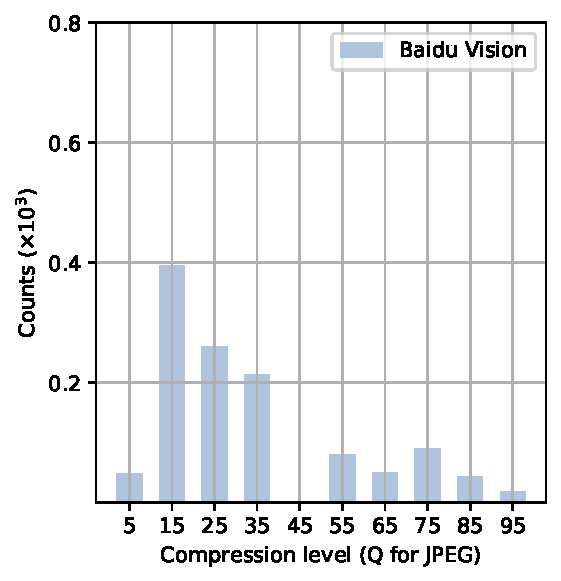
\includegraphics[width=4.8cm]{figures/ImageNet_Baidu_choices1.pdf}}
		\centerline{(a) Baidu Vision}
	\end{minipage}
	\hfill
	\begin{minipage}[t]{0.32\linewidth}
		\centerline{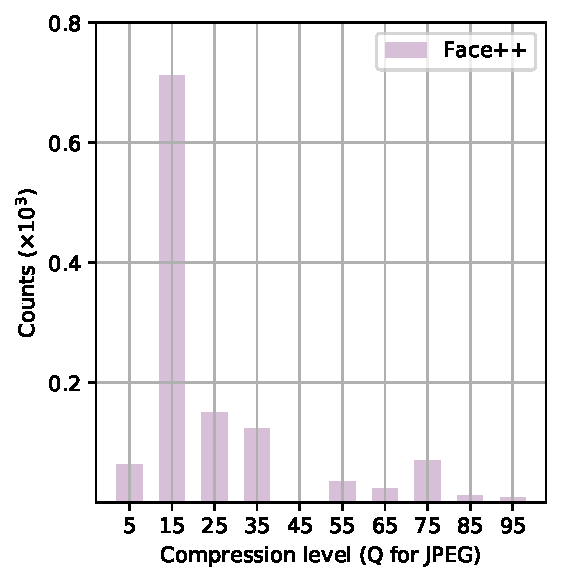
\includegraphics[width=4.8cm]{figures/ImageNet_Facepp_choices1.pdf}}
		\centerline{(b) Face++}
	\end{minipage}
	\hfill
	\begin{minipage}[t]{0.32\linewidth}
		\centerline{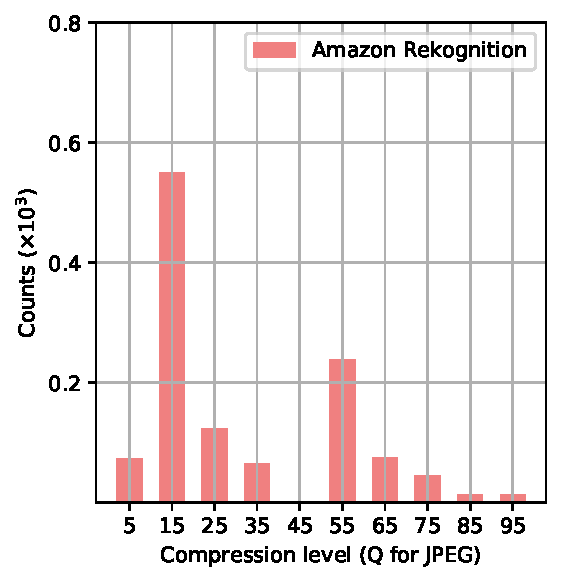
\includegraphics[width=4.8cm]{figures/ImageNet_Amazon_choices1.pdf}}
		\centerline{(c) Amazon Rekognition}
	\end{minipage}		
	\caption{\textcolor{revise}{Histogram of RL agent's best compression quality level selection for different cloud services}}
	\label{fig: quality_chosen}
}
\end{figure*}

%\begin{figure}[!t]
%	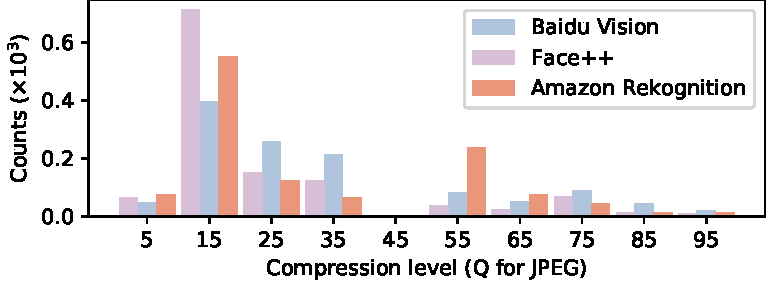
\includegraphics[width=0.8\linewidth]{figures/quality_chosen.pdf}
%	\caption{Histogram of RL agent's best compression quality level selection for different cloud services}
%	\label{fig: quality_chosen}
%	% \vspace{-0.3cm}
%\end{figure}

Moreover, in our experiment, the agent presents different behaviors when the input image changes from one dataset to another. Figure~\ref{fig: dataset_change} shows the agent's choices for the same backend cloud model (Baidu Vision) but different image datasets. We prepare two datasets indicating two contextual ``sceneries''. We randomly sample images from ImageNet~\cite{ImageNet} whose images are mostly taken in the daytime, to act as a daytime scenery, and randomly select nighttime images from the FLIR Thermal Dataset~\cite{FLIR} to form another dataset to act as a nighttime scenery. \textcolor{revise}{The histogram shown in Figure~\ref{fig: dataset_change} points out that the distribution of compression quality levels is different on ImageNet and FLIR Thermal Dataset. For ImageNet and FLIR, the mean is respectively 43.3 and 47.5, and the standard deviation is respectively 19.52 and 26.56.} We can see that, to maintain high accuracy, when the input image's contextual group $ \mathcal{X} $ changes, the agent's compression quality level selection would change as well. This phenomenon presents that the agent can adaptively choose a proper compression quality level based on the input image's features. 

\textcolor{revise}{We can also find that Figure~\ref{fig: quality_chosen}(a) and Figure~\ref{fig: dataset_change}(a) is different, even if we use the same cloud service (Baidu Vision) and image dataset (ImageNet). When we use the same cloud service at different times, the cloud service commonly invokes different backend cloud models. Therefore the interaction between the agent and the backend cloud model is different. This result variation presents that the agent can adaptively make a proper compression strategy in different complex environments, indicating our solution's generality and practicality.} %% \\

%The histogram shown in Figure~\ref{fig: dataset_change} points out that, for the ImageNet images, the agent prefers a low compression quality level, but its choices are distributed more evenly. For the FLIR Thermal images, the agent's choices are more accumulated in some relatively higher compression quality levels.

%\begin{figure}[!t]
%    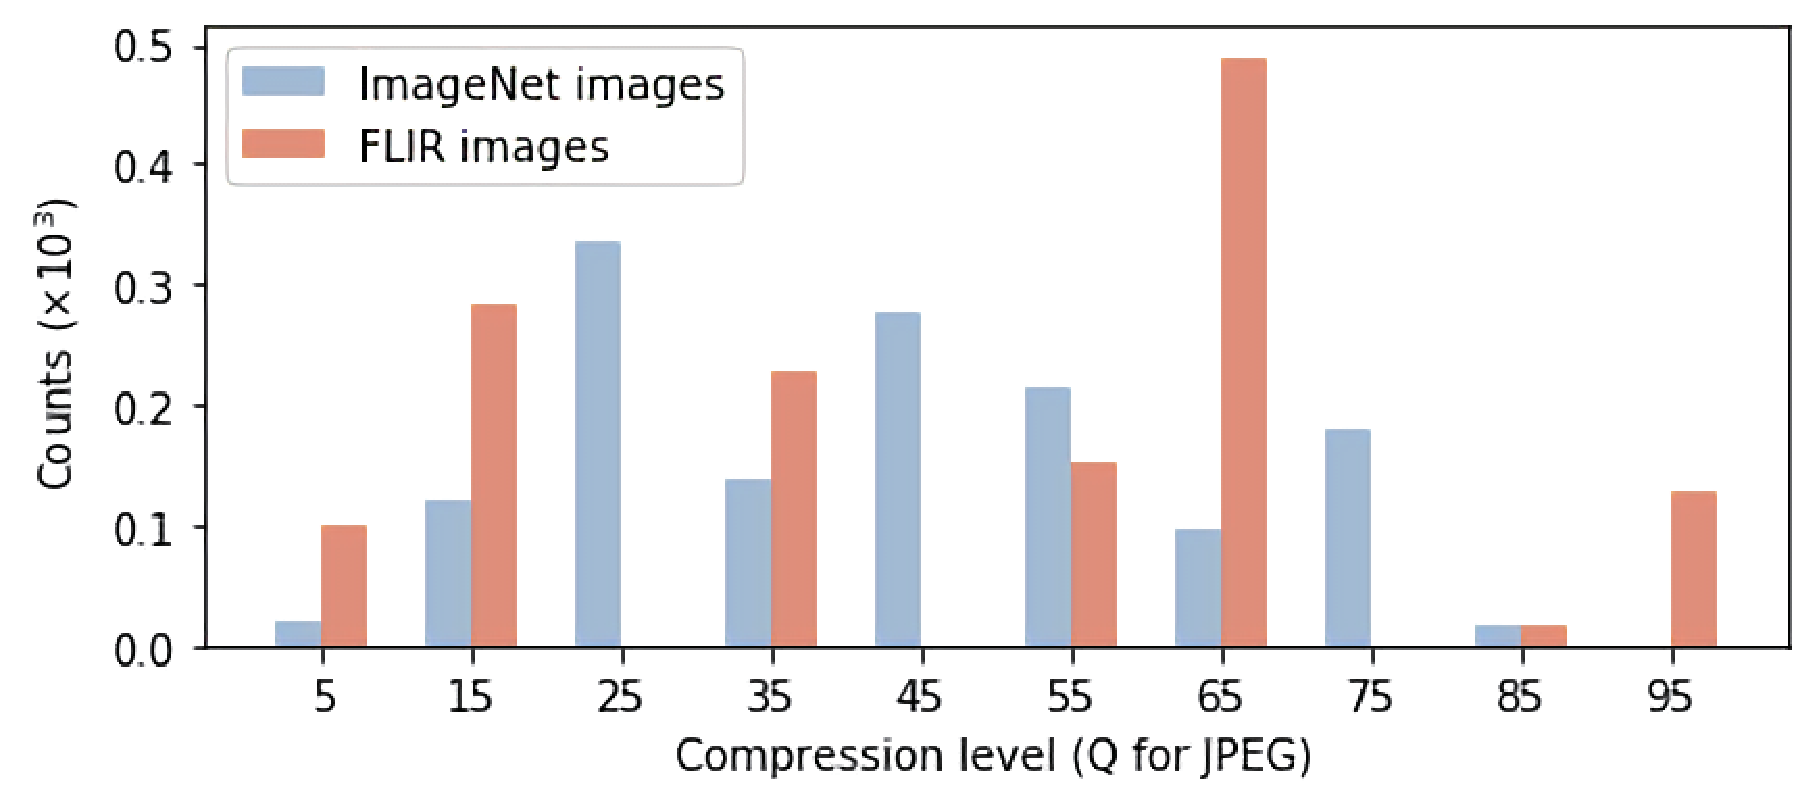
\includegraphics[width=0.8\linewidth]{figures/dataset_change.pdf}
%    \caption{Histogram of RL agent's best compression level selection for different scenery image inputs}
%    \label{fig: dataset_change}
%\end{figure}

\begin{figure*}[!t]
{\color{revise}
	\begin{minipage}[t]{0.48\linewidth}
		\centerline{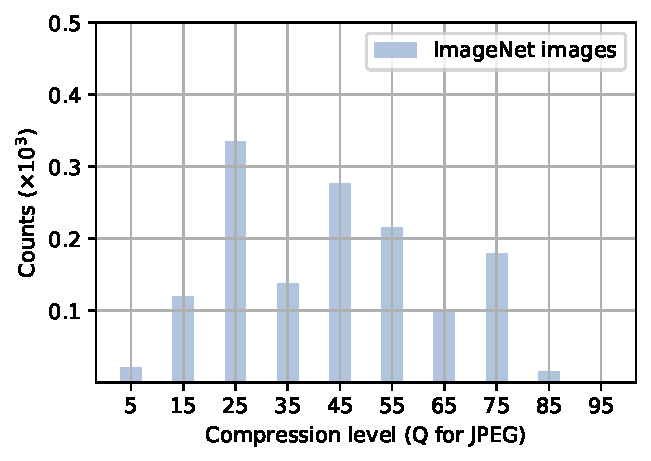
\includegraphics[width=7cm]{figures/ImageNet_Baidu_choices.pdf}}
		\centerline{(a) ImageNet images}
	\end{minipage}
	\hfill
	\begin{minipage}[t]{0.48\linewidth}
		\centerline{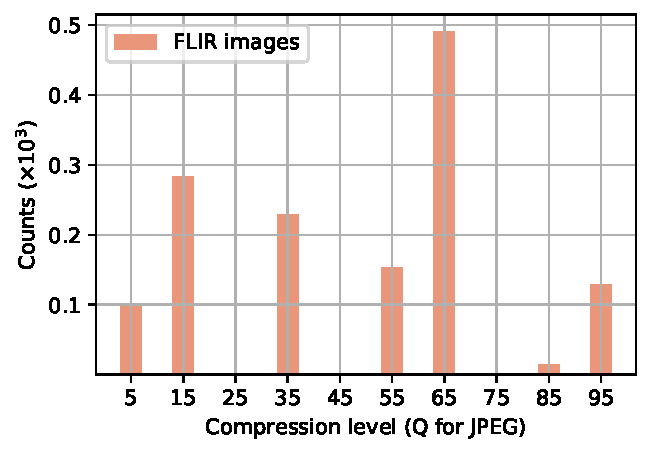
\includegraphics[width=7cm]{figures/FLIR_Baidu_choices.pdf}}
		\centerline{(b) FLIR images}
	\end{minipage}	
    \caption{\textcolor{revise}{Histogram of RL agent's best compression quality level selection for different scenery image inputs}}
	\label{fig: dataset_change}
}
\end{figure*}

%\subsubsection{\textbf{Attention Map Variation}}
\subsubsection{Attention Map Variation:}
\label{subsec: attention map}

To make insight investigations, we plot the importance map of a chosen compression quality level. We leverage a conventional visualization algorithm, Grad-Cam, to observe the Deep Q-Learning Network-based agent's interest when choosing compression quality levels. Grad-Cam is a widely used effective solution to present the importance map of a deep neural network by calculating the gradients of each target concept and backtracking to the final convolution layer. In this work, we plot the RL agent's attention map by Grad-Cam in Figure~\ref{fig: attention}. %% \\

\begin{figure*}[!t]
	\begin{minipage}{0.2\linewidth}
		\centerline{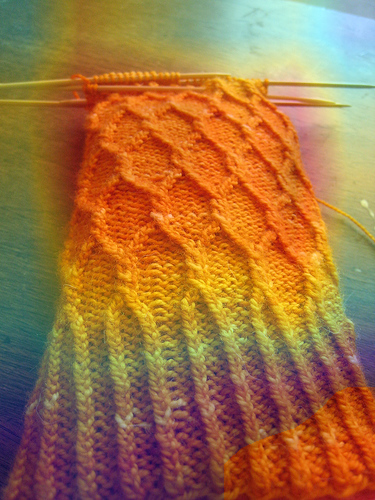
\includegraphics[width=3.5cm, height=3.0cm]{figures/robust_figure1.png}}
		\centerline{(1a) Q=5}
	\end{minipage}
	\hfill
	\begin{minipage}{0.2\linewidth}
		\centerline{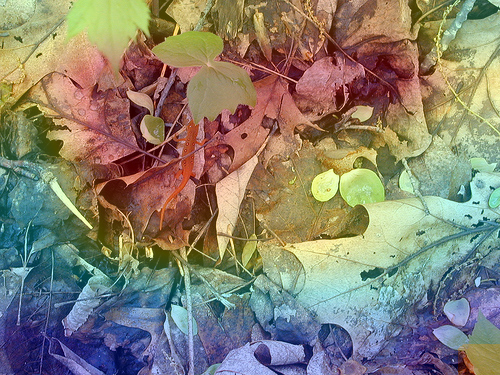
\includegraphics[width=3.5cm, height=3.0cm]{figures/robust_figure2.png}}
		\centerline{(1b) Q=15}
	\end{minipage}
	\hfill
	\begin{minipage}{0.2\linewidth}
		\centerline{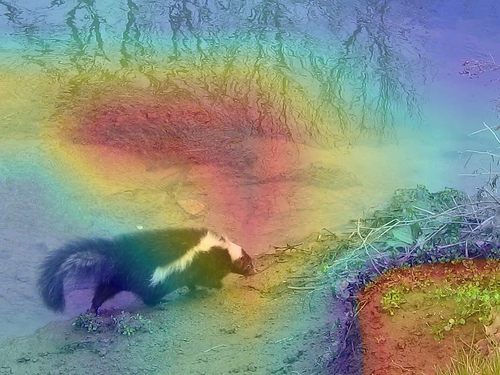
\includegraphics[width=3.5cm, height=3.0cm]{figures/robust_figure3.png}}
		\centerline{(1c) Q=15}
	\end{minipage}
	\hfill
	\begin{minipage}{0.2\linewidth}
		\centerline{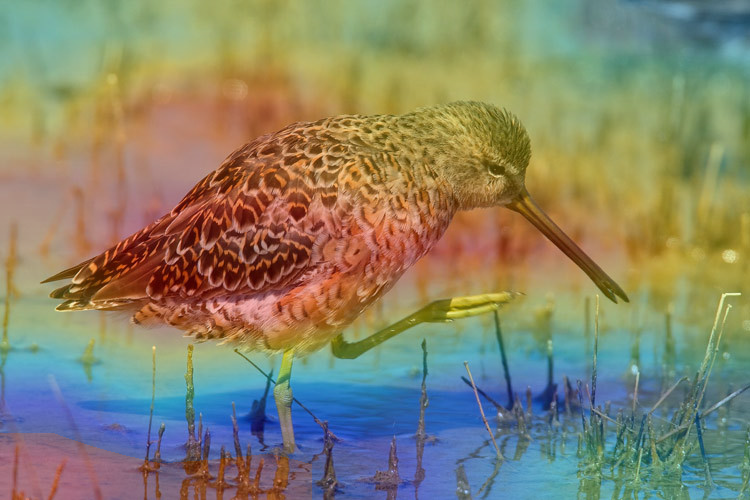
\includegraphics[width=3.5cm, height=3.0cm]{figures/robust_figure4.png}}
		\centerline{(1d) Q=15}
	\end{minipage}
	
	\vfill
	\vspace{0.4cm}
	
	\begin{minipage}{0.2\linewidth}
		\centerline{
\includegraphics[width=3.5cm, height=3.0cm]{figures/sensetive_figure1.png}}
		\centerline{(2a) Q=85}
	\end{minipage}
	\hfill
	\begin{minipage}{0.2\linewidth}
		\centerline{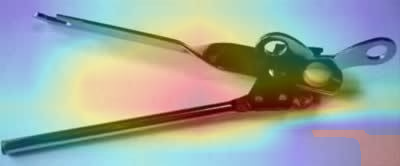
\includegraphics[width=3.5cm, height=3.0cm]{figures/sensetive_figure2.png}}
		\centerline{(2b) Q=85}
	\end{minipage}
	\hfill
	\begin{minipage}{0.2\linewidth}
		\centerline{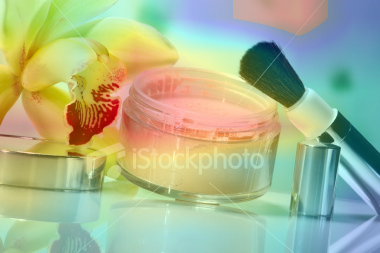
\includegraphics[width=3.5cm, height=3.0cm]{figures/sensetive_figure3.png}}
		\centerline{(2c) Q=75}
	\end{minipage}
	\hfill
	\begin{minipage}{0.2\linewidth}
		\centerline{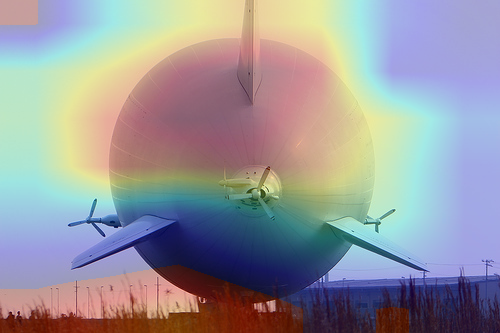
\includegraphics[width=3.5cm, height=3.0cm]{figures/sensetive_figure4.png}}
		\centerline{(2d) Q=75}
	\end{minipage}
%	\vspace{0.2cm}
	\caption{Visualization of the importance map for the RL agent to choose a compression quality level}
	\label{fig: attention}
\end{figure*}

In our investigations, we find that in different environments $ \{\mathcal{X}, M\} $, the RL agent selects compression quality levels based on the visual textures of different regions in the image. As shown in Figure~\ref{fig: attention}, picture 1a -- 1d are some pictures which the agent chooses to compress aggressively. The agent selects low compression quality levels based on the complex texture of the images. On the contrary, for pictures 2a -- 2d, the agent chooses relatively higher compression quality levels to preserve more details since its interest falls on some smooth regions. Especially for 1a and 2a, for picture 1a, the agent chooses a low compression quality level based on the rough central region though there are smooth regions around it, for picture 2a, the agent chooses a relatively higher compression quality level based on the surrounding smooth region rather than the central region. %% \\